\documentclass[times, utf8, diplomski, english]{fer}
\usepackage{booktabs}
\usepackage[hidelinks]{hyperref}
\usepackage{footnote}
\usepackage{graphicx}
\usepackage{mathtools}

\usepackage{listings}
\usepackage{protobuf/lang}  % include language definition for protobuf
\usepackage{protobuf/style} % include custom style for proto declarations.

\DeclareMathOperator*{\argmin}{\arg\!\min}
\DeclareMathOperator*{\argmax}{\arg\!\max}
\graphicspath{ {./figures/} }

\begin{document}

\thesisnumber{1572}
\title{ End-to-End Deep Learning Model for Base Calling of MinION Nanopore Reads}
\author{Neven Miculinić}
\maketitle
 
\izvornik

\zahvala{I would like to thank my mentor, Mile Šikić, for his patient guidance, encouragement
    and advice provided over the years.
    
I would also like to thank my family and friends for their
    continuous support.
    
In the end, honorable mentions go to Marko Ratković for his help with this thesis.	
}

\tableofcontents
\listoffigures
\listoftables

%%%%%%%%%%%%%%%%%%%%%%%%%%%%%%%%%%%%%%%%%
% Chapter Introduction
%%%%%%%%%%%%%%%%%%%%%%%%%%%%%%%%%%%%%%%%%
\chapter{Introduction}
\label{chap:Introduction}
In recent years, deep learning methods significantly improved the state-of-the-art in multiple domains such as computer vision, speech recognition and natural language processing~\citep{LeCun:1998:CNI:303568.303704, NIPS2012_4824}
In this paper, we present application of deep learning for DNA basecalling problem.

Oxford Nanopore Technology's MinION nanopore sequencing platform~\cite{mikheyev2014first} is the first portable DNA sequencing device. It produces longer reads than competing technologies. In addition, it enables real-time data analysis which makes it suitable for various applications.
Although MinION is able to produce long reads, even up to 882 kb~\cite{loman1-100k,loman2-800k}, they have an error rate of 10\% or higher. This master thesis uses R9.4 pore model and compares previous techniques with novel auto-encoder multi-task training. 

\section{Organization}
[TODO]: Write some fancy stuff once completed.

%%%%%%%%%%%%%%%%%%%%%%%%%%%%%%%%%%%%%%%%%
% Chapter Background
%%%%%%%%%%%%%%%%%%%%%%%%%%%%%%%%%%%%%%%%%

\chapter{Background}
\label{chap:background}
Due to technical constraints, it's infeasible  to sequence whole DNA in single strand. 
Every sequencing technology to date have an upper limit how big strand can it precisely sequence.
This limit is considerably smaller than size of genome.
For example E.Coli has ~4.5 million base pairs in its DNA, while Sanger's sequencing maximum output is around 1000 base pairs max.
To make DNA basecalling feasible technique called shotgun sequencing was invented. 
The strand is cloned number of times, then via chemical  agent broken down into smaller fragments of appropriate length. 
Sequenced fragments are called reads.

Genome assembly is the process of reconstructing the original genome from reads and usually starts with finding overlaps between reads.
The quality of reconstruction heavily depends on the length and the quality (accuracy) of the reads produced by the sequencer. 

If we have reference sequence we usually align the reads on the reference to aid us into genome assembly. Otherwise we have to use many de novo assembly techniques.

The right analogy would be building a puzzle. Since we cannot scan the whole puzzle because our camera is too small or imprecise, we are scanning pieces of the whole picture. Puzzle pieces would represent fragments in this analogy. If we have a map, even a rough one, it shall aids us into assemblying those puzzle pieces into complete pictures. Otherwise we're fiddling in the dark and using de novo assembly techniques.

Figure \ref{fg:sequencing} depicts process of sequencing visually.

\begin{figure}[!ht]
    \begin{center}
        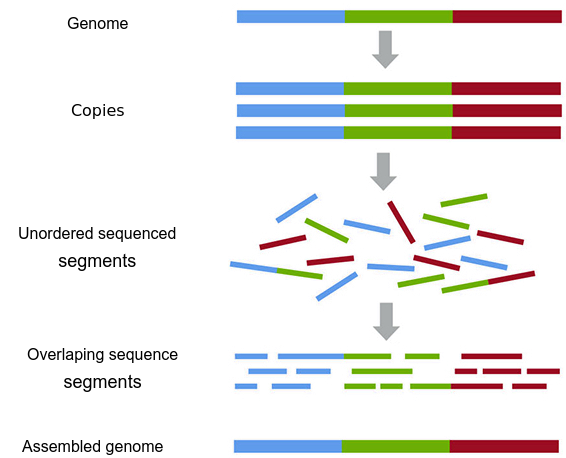
\includegraphics[width=0.6\textwidth]{shotgun-sequencing}
        \caption{Depiction of the sequencing process}
        \label{fg:sequencing}
    \end{center}
\end{figure}


In 1977, Frederick Sanger~\citep{mile}\citep{Pettersson2009} started development of sequencing technologies. It allowed read lengths up to 1000 bases with very high accuracy(99.9\%) at the cost of 1\$ per 1000 bases.
Later, seconds generation sequencing, like IAN Torrent and Illumina devices, reduced the price while keeping the accuracy high. However, they had a cost of shorter read lengths, about a few hundred base pairs, which makes resolving repetitive regions practically impossible.

Third generation sequencing technologies have longer read lengths at the accuracy's expense. PacBio, for example, developed technology with a few thousand bases with error rates of \textasciitilde10-15\%. 

MinION sequences, which this master thesis use, made sequencing less expensive and even portable.

\section{Oxford Nanopore MinION}

The MinION device by Oxford Nanopore Technologies is the first portable DNA sequencing device. Its small weight, low cost, and long read length combined with decent accuracy yield promising results in various applications including full human genome assembly \cite{human_seq} what could potentially lead to personalized genomic medicine. It weights only 87 grams, and its portability lead to uses on international space station and the antarctic among other places.

Under the hood, it has numerous nano-meter sized pores, thus a names Nanopore. Each pore has width of around 6 nucleotied. Under electric current DNA strand passed through the pore and changes its electric resistance. The sensor measures current through the pore multiple times a second~\footnote{The model we worked with had 4000 samples per seconds}. This signal varies depending which k-mer is occupying the pore, and on its basis we're performing the basecalling. On figure~\ref{fg:nanopore} this process is visually depicted. 

MinION devices can produce long reads, usually tens of thousand base pairs (with reported reads lengths of 100 thousand \cite{loman1-100k} and even recently above 800 thousand base pairs \cite{loman2-800k}), but with high sequencing error than older generations of sequencing technologies.

\begin{figure}[!ht]
    \begin{center}
        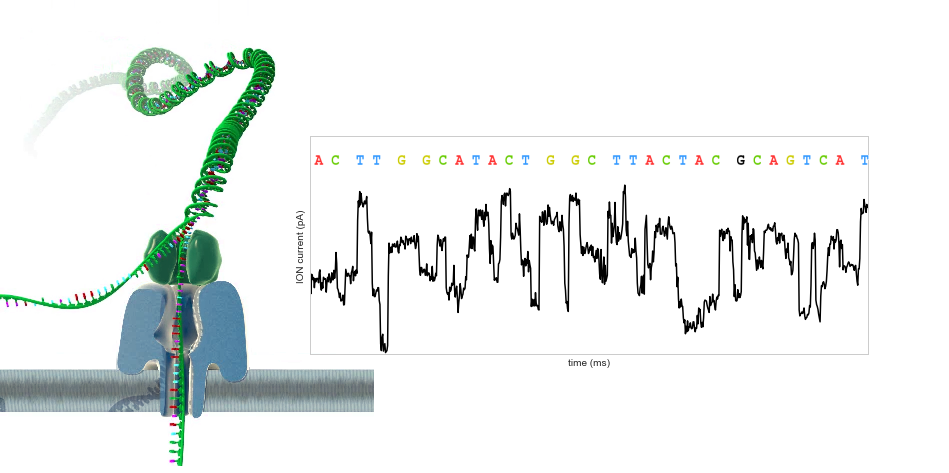
\includegraphics[width=0.7\textwidth]{nanopore}
        
        \caption[DNA strain being pulled through a nanopore]{DNA strain being pulled through a nanopore \protect\footnotemark}
        \label{fg:nanopore}
    \end{center}
\end{figure}
\footnotetext{Figure adapted from https://nanoporetech.com/how-it-works}

The sequecing resulting file is in FAST5 format, which is adapted HDF5 file format, popular in bioinformatics community. It stores raw signal, alongside various metadata. Unfortunately, many basecallers, including the official ones, upon executing store their results in the FAST5 files. It leads to data and processing coupling in single file, and bloated file sizes. 

\begin{figure}[!ht]
    \begin{center}
        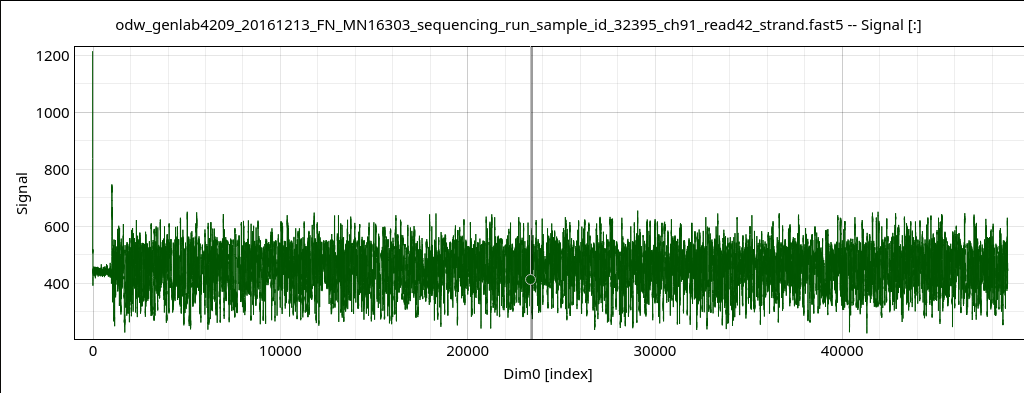
\includegraphics[width=0.6\textwidth]{fast5_sample}
        \caption[Structure of FAST5 file and raw signal plot show in \textit{HDFView}]{Structure of FAST5 file and raw signal line plot show in \textit{HDFView} \protect\footnotemark}
        \label{fg:fast5}
    \end{center}
\end{figure}
\footnotetext{https://support.hdfgroup.org/products/java/hdfview/}
  
\section{Related work}

\subsection{Oxford Nanopore Technologies}
This subsection covers various basecallers published by ONT, the MinION device maker.
\subsubsection{Metrichor}

Metrichor is now defunct cloud based basecaller. The older versions used \textit{hidden Markov models} (HMM) as underlying algorithm. Preprocessing started with segmenting signal into smaller chunks called events with their start, end, length, mean signal strength and standard deviation. This events are observations in the HMM model, and the underlying generating hidden sequence is sequence of 6-mers. They build their HMM transition matrix with stay, skip 1 and skip 2 probabilities, that is underlying 6-mer cannot move for more than 2 nucleotides per event. Basecalling is performed using Viterbi algorithm. This approach showed poor results when calling long homopolymer stretches as the context in the pore remains the same \cite{homopolymers}\cite{homopolimeri_analiza}.

\subsubsection{Nanonet}
Nanonet is ONT first generation neural network basecaller. It used to be available on github, but it's now defunct and unavailable.

\subsubsection{Albacore}
Albacore is a production basecaller provided by Oxford Nanopore, and uses a command-line interface. It
utilizes the latest in Recurrent Neural Network algorithms in order to interpret the signal data from the
nanopore, and basecall the DNA or RNA passing through the pore. It implements stable features into
Oxford Nanopore Technologies’ software products, and is fully supported. It receives .fast5 files as an
input, and is capable of producing: 
\begin{itemize}
    \item .fast5 files appended with basecalled information
    \item .fast5 files that have been processed, but basecall information present in a separate .fastq file
\end{itemize}

\subsubsection{Guppy}
Guppy is ONT's new basecaller that can use GPUs to basecall much faster than Albacore. Both the GridION X5 and PromethION contain GPUs and use Guppy to basecall while sequencing. Guppy can also use CPUs and scales well to many-CPU systems, so it may run faster than Albacore even without GPUs.  In the future it's intended to replace Albacore as production basecaller.
\subsubsection{Scrappie}
Scrappie\footnote{\url{https://github.com/nanoporetech/scrappie}} is ONT's research basecaller. Scrappie is reported to be the first basecaller that specifically address homopolymer base calling. It became publicly available just recently in June, 2017 and supports R9.4 and future R9.5 data.

Unlike Albacore, Scrappie does not have fastq output, either directly or by writing it into the fast5 files – it only produces fasta reads.

\subsection{Third-party basecallers}

\subsubsection{Nanocall}
Nanocall~\citep{David046086} was the first third-party open source basecaller for nanopore data. It uses HMM approach like the original R7 Metrichor. Nanocall does not support newer chemistries after R7.3.

\subsubsection{DeepNano}
DeepNano~\citep{Boza2017}  was the first open-source basecaller based on neural networks. It uses bidirectional recurrent neural networks implemented in Python, using the Theano library. When released, originally only supported R7 chemistry, but support for R9 and R9.4 was added recently.
\subsubsection{basecRAWller}
basecRAWller~\footnote{\url{https://basecrawller.lbl.gov/}} is developed by Marcus Stoiber and James Brown at the Lawrence Berkeley National Laboratory.

\subsubsection{Chiron}
Chiron~\citep{chiron_teng} is developed by Haotian Teng and others in Lachlan Coin's group at the University of Queensland. They are basecalling from the raw signal, using first residual convolutional neural network, than LSTM and finally beam search or greedy decoder depending on chosen configuration. 

\chapter{Methods}
\label{chap:methods}
This chapter is dedicated to explaining key deep learning concepts used throughout the master thesis. It's here primarily for completeness, and it's author recommendation to go into detail via other sources, for example Deep learning book~\citep{deep_learning_book-Goodfellow-et-al-2016}, google, or research papers cited for most of the techniques.. TensorFlow~\citep{tensorflow2015-whitepaper} and Keras~\citep{chollet2015keras} deep learning frameworks were used for implementation. For each deep learning concept I'll provide equivalent keras/tensorflow code whichever one is simpler and used throughout the codebase.

\section{Neural Network}
Feed-forward Neural network is the basic building block of any deep learning system. It's composition of multiple differentiable functions. Commonly we have input vector $x$, apply some linear transformation to it and add bias, and finally on the result some activation function. Details on common choices for actionvation function are in section~\ref{sec:activation}. In mathematical language $y = f(Ax + b)$ would be one layer of neural network transforming input $x$ into output $y$. Stacking those operation we get multiple layers, hence the word deep in deep learning. Simple 3-layer neural network is depicted in figure~\ref{fg:nn}.

\begin{figure}[!ht]
    \begin{center}
        \begin{align*}
            y_1 &= f(A_1x + b_1) \\
            y_2 &= f(A_2y_1 + b_2) \\
            y &= f(A_3y_2 + b_3) \\
        \end{align*}
        \caption{Simple three layer feed forward neural network}
        \label{fg:nn}
    \end{center}
\end{figure}

\section{Activation functions}
\label{sec:activation}

Most neural network operations are linear transformation. Composing multiple linear transformation we get new linear transformation. Thus have non-linear behavior we use the non-linear activation functions. Originally, the most popular choice was $\tanh$ and $\sigma(x) = \frac{1}{1 + e^{-x}} $ activation functions. They are nice because of limited output domain. 

However, other choices proved more effective, especially with deep neural network due to greater learning speeds, and to overcome gradient vanishing problem. Gradient vanishing refers to neural network gradient approaching zero as we back propagate through more and more layers. Exploding gradient is related phenomena in which gradient approaches infinity. Both present serious hampering to neural network training.

ReLU, The rectified linear unit, $f(x) = \max(0, x)$,  is one hugely popular choice and decent baseline compared to other ReLU variants. ReLU greatly accelerates the convergence of stochastic gradient descent compared to $\sigma$ and $\tanh$ activation functions~\citep{NIPS2012_4824}. 

Furthermore, its calculation is drastically simpler then computing transcendental functions, like $\sigma$ or $\tanh$.

Over time, ReLU showed its downsides, called \textit{dying ReLU}. It still saturates the gradients when it's 0, that is when $x <= 0$ giving no useful gradient to back propagate. Thus several ReLU variant have been proposed: PrRelu~\citep{prelu} in equation~\ref{eq:prelu}, ELU~\citep{elu} in equation~\ref{eq:elu}, and finally SeLU~\citep{selu} in equation~\ref{eq:selu}. In Selu constants $\alpha$ and $\lambda$ are chosen in such a way that output gravitates towards normal distribution with zero mean and unit variance. Those constants are: $\lambda = 1.0507$ and $\alpha = 1.6732$. 
Code generating the function plot is displayed in figure~\ref{fg:actcode}, and the plot is in figure~\ref{fg:act_plot}

\begin{equation}    
\label{eq:prelu}
PrELU(x)=
\begin{cases}
x & \text{if}\ x>0 \\
\alpha x & \text{otherwise}
\end{cases}\\
\end{equation}

\begin{equation}
\label{eq:elu}
ELU(x)=
\begin{cases}
x & \text{if}\ x>0 \\
\exp(x) - 1 & \text{otherwise}
\end{cases}    \\
\end{equation}

\begin{equation}
\label{eq:selu}
\text{selu}(x)= \lambda
\begin{cases}
x & \text{if}\ x>0 \\
\alpha e^x - \alpha & \text{otherwise}
\end{cases} 
\end{equation}

\begin{figure}
\begin{lstlisting}[language=python,style=protobuf]
import tensorflow as tf
import keras
import seaborn as sns
import numpy as np
import matplotlib.pyplot as plt

for act in ["relu","selu", "elu"]:
    with tf.Graph().as_default():
        x = tf.placeholder(shape=(None, ), dtype=tf.float32)
        y = keras.layers.Activation(act)(x) 

        with tf.Session() as sess:
            xx = np.linspace(-1, 1)
            yy = sess.run(y, feed_dict={
                x: xx
            })
            plt.plot(xx, yy, label=act)
            plt.legend()
\end{lstlisting}
\label{fg:actcode}
\caption{Code generating the activation function plot. Also shows how tensorflow and keras could be used}
\end{figure}

\begin{figure}
    \begin{center}
        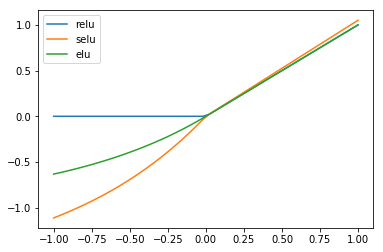
\includegraphics[width=0.8\textwidth]{act_plot}
        \caption{Plot of common activation functions between -1 and 1. PrELU is excluded since the parameter $\alpha$ is learnt during training}
        \label{fg:act_plot}
    \end{center}
\end{figure}

\section{CNN}
Convolutional Neural Networks(CNNs) are the bread and butter of almost all computer vision system today, and they lunched the deep learning hype with unprecedented results on Image Classification problems. 
Lately, their scope is expanded to Natural language processing (NLP) tasks with promising results~\citep{BYTENET, facebook}.

Convolution is a type of feed-forward neural network layer where the weights are tied together. We have a sliding window over which we apply linear transformation of the input, and get the output element. This operation is repeated to get the full output tensor. For 1D case~\footnote{\url{https://keras.io/layers/convolutional}} figure~\ref{fg:convolution} depicts it visually. 

There's also atrous convolution~\cite{atrous_DBLP:journals/corr/ChenPSA17}, also known as dilated convolution where spaced input tensor elemets are taken depending on the dilation factor. Ordinary convolution is a special case with $\text{dilation} = 1$.

\begin{figure}
	\begin{center}
		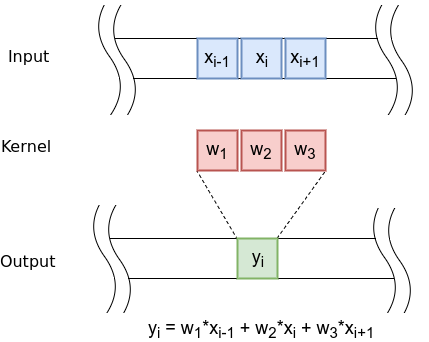
\includegraphics[width=0.5\textwidth]{convolution}
		\caption{Convolution layer, kernel size 3 with stride 1. Adapted from~\citep{mratkovic} with authors permission.}
		\label{fg:convolution}
	\end{center}
\end{figure}

\section{RNN}
RNN, residual neural networks are one of the basic building blocks in sequence models. They are feed-forward neural netwoek spanned in time domain. The same neural network is applied to two inputs, hidden state and input at time $t$ and gives two outputs, new hidden state and output at time $t$. The historic information remains saved in the hidden state, and it's propagated to the future. It's visual description is depicted in figure~\ref{fg:rnn}.

\begin{figure}[!ht]
    \begin{center}
        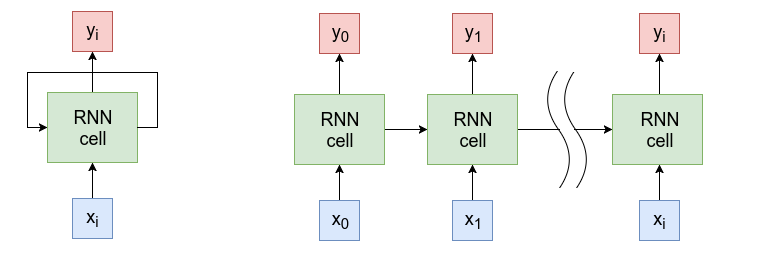
\includegraphics[width=0.8\textwidth]{rnn}
        \caption{An unrolled recurrent neural network. Adapted from~\citep{mratkovic} with authors permission.}
        \label{fg:rnn}
    \end{center}
\end{figure}


They can be unrolled in one massive feed-forward neural network. They are trained with backpropagation through time, on this unrolled graph. Usually the unrolling is capped and fixed number or time steps. 
Common issue to vanilla RNNs is vanishing and exploding gradients problem. It's solved by redesigning the basic RNN cell. There are two common approaches called LSTM~\citep{hochreiter1997long} and GRU~\citep{gru}.

Bidirectional Recurrent Neural (BiRNN) networks are used when the current output not only depends on the previous elements in the sequence but also future elements. Basically we're stacking to RNNs, one in forward direction and another in the backward and concatenating the hidden states/outputs. This approach was used in DeepNano~\citep{Boza2017}.

Despite their modeling power, main drawback is their speed. Since they are processing data sequentially, it's hard to paralize those operations. 

\section{Pooling layer}
Pooling layers refer to tensor dimensionality reduction. Tensor is squeezed by some factor, and each block of factor width is aggregated using some aggregation function. 
In other words, we divide our tensor into equally shaped hyperrectanges, and each aggregate using aggregation function yielding new hyperrectange. 
Fox example, maxPool2d for  image sized 50x50 shall with pool size (2,2) shall divide it into rectangles of size (2, 2) max those 4 elements and result in image sized 25x25.
This is visually depicted in figure~\ref{fg:fg:maxpool}.
Common choices are AvgPool, and MaxPool~\citep{Scherer:2010:EPO:1886436.1886447}~\footnote{\url{https://keras.io/layers/pooling/}}.

\begin{figure}[!ht]
    \begin{center}
        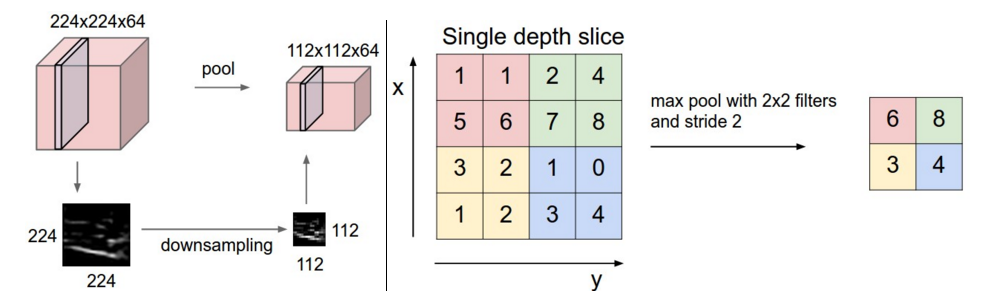
\includegraphics[width=0.8\textwidth]{Pooling_Simple_max}
        \caption{Example of max pool layer in convolutional neural network. Adapted from~\url{https://leonardoaraujosantos.gitbooks.io/artificial-inteligence/content/pooling_layer.html}}
        \label{fg:maxpool}
    \end{center}
\end{figure}

\chapter{System architecture}
\section{Data Preparation}

In previous project incarnation, we used fast5 with additional custom .ref files as our dataset. This setup had some issues. First, it was IO heavy since we were reading the whole fast5 file which contained non-raw data section~\footnote{like basecalling from other basecallers}, data management with separated raw files and labels, and lastly it was a magic to parse it every time. Which exactly group or subgroup within fast5, or is the signal start normalized to 0, or is it some arbitary begging written at some other place in fast5 files changes from version to version. 

Therefore, for this project I've decided to make my own custom format for training described via protobuf~\citep{protobuf}. The issue from previous versions weren't the only reason. Another was ease of importing other peoples data in their formats into this one. If I can read it, I can easily write plugin converting between formats. As of writing this thesis 4 such plugins were written since I wasn't sure which data I shall use and in which format am I going to import them in. 

Ease of machine encoding/decoding as well as other previously mentioned factors guided this decision. Also I've written written datapoint format inspector operating on this common format, making my life easier. The source code for conversion procedures can be found on minion-data~\footnote{\url{https://github.com/nmiculinic/minion-data}} github repository as well as pypi. The specific interface description language(IDL) can se seen in figure~\ref{fg:dataset_proto}.


\begin{figure}
    \begin{center}
    \begin{lstlisting}[language=protobuf3,style=protobuf]
syntax = "proto3";

package dataset;

enum BasePair {
    A = 0;
    C = 1;
    G = 2;
    T = 3;
    BLANK = 4;
}

enum Cigar {
    MATCH = 0;
    MISMATCH = 1;
    INSERTION = 2; // Insertion, soft clip, hard clip
    DELETION = 3;  // Deletion, N, P
}

message DataPoint {
    message BPConfidenceInterval {
        uint64 lower = 1;
        uint64 upper = 2;
        BasePair pair = 3;
    }
    repeated float signal = 1;
    repeated BasePair basecalled = 2; // What we basecalled
    repeated BPConfidenceInterval labels = 3; // labels describe corrected basecalled signal for training
}
    \end{lstlisting}
    \caption{dataset protobuf description}
    \label{fg:dataset_proto}
    \end{center}
\end{figure}

Data has been downloaded from \url{https://data.genomicsresearch.org/Projects/online_dataset/train_set_all/}.  The following species were provided there by the Chiron team:
\begin{itemize}
    \item Human
    \item E. Coli
    \item Lambda Phage
\end{itemize}

For the concrete Chiron dataset, the re-squiggled preparation method was used. (The data was re-squiggled, that is after aligning the read on the reference, the read data is improved and each base pairs place on the raw signal is calculated.)

The re-squiggled basecalled data is located at \verb|/Analyses/RawGenomeCorrected_000/BaseCalled_template/Events|. The interesting code fragments are in function processDataPoint of file \verb|minion_data/preperation/_re_squggled.py| from minion-data python package.

After the gzipped dataset is prepared, it goes into the training pipeline. The whole training \& testing pipeline is available  open source on \url{https://github.com/nmiculinic/minion-basecaller}

\section{Training pipeline}
After getting data in uniform format, the training part comes next. In aiming this as observable and simple as possible I've modeled config in using python3 \texttt{typing.NameTuple}~\footnote{\url{TODO}} and volptous for data validation. 
With those two tools I've created statically typed configuration file format and data validation with human readable error. As serialization format I've chosen YAML for it's readability and tersness. 
The config file definiton is in figure~\ref{fg:train_cfg_py} and example config file for training is in figure~\ref{fg:train_cfg_yml}. The source code can be found in module \texttt{mincall.train.\_train.py} and we're recommending reading it for extended details.

\begin{figure}
    \begin{center}
    \begin{lstlisting}[language=python,style=protobuf]
class TrainConfig(NamedTuple):
    model_name: str
    train_data: List[DataDir]
    test_data: List[DataDir]
    logdir: str
    seq_length: int
    batch_size: int
    surrogate_base_pair: bool

    train_steps: int
    init_learning_rate: float
    lr_decay_steps: int
    lr_decay_rate: float

    model_hparams: dict = {}
    grad_clipping: float = 10.0
    validate_every: int = 50
    run_trace_every: int = 5000
    save_every: int = 2000

    tensorboard_debug: str = ""  # Empty string is use CLI debug
    debug: bool = False
    trace: bool = False

    @classmethod
    def schema(cls, data):
        return named_tuple_helper(
            cls, {
                'train_data': [DataDir.schema],
                'test_data': [DataDir.schema],
            }, data
        )

    \end{lstlisting}
    \caption{dataset protobuf description}
    \label{fg:train_cfg_py}
    \end{center}
\end{figure}

\begin{figure}
    \begin{center}
    \begin{lstlisting}[]
version: "v0.1"
train:
  train_data:
    - name: "r9.4"
      dir: "./mincall/example"
  test_data:
    - name: "r9.4"
      dir: "./mincall/example_test"
  model_name: "dummy"
  model_hparams:
    num_layers: 5
  surrogate_base_pair: false
  train_steps: 60
  init_learning_rate: !!float 1e-4
  lr_decay_steps: 10000
  lr_decay_rate: 0.5
  seq_length: 40
  batch_size: 10
  logdir: "./logs"
    \end{lstlisting}
    \caption{dataset protobuf description}
    \label{fg:train_cfg_yml}
    \end{center}
\end{figure}

Input data is read via background thread which processes it, packages it into signal and label slices, and pushed into tensorflow space queues. Inside those queues, data is shuffled, and composed into batched for further training. This part of the code has extensive test suide, including end2end test with golden file~\footnote{golden ftextile is test technique where you save function output to golden file, verify manually it's correct, and after each successing test you're checking that nothing changed. This way we can be sure refactoring didn't influence correctness.}

From configuration rest of the pipeline is initialized. This included model, with its hyperparameters, loading config defined train and test sets, learning rate schedule, sequence lengths, batch size and other settings. Keras is used for model definition due to its simplicity in design. 

Additionally I've embedded edlib [TODO] CITE EDLIB.
in the tensorflow \texttt{tf.py\_func} operator which enabled me having match, mismatch, insertion, deletion and identiry rates observer during training on both train and test set.

Standard python logging module was used with multiple backends. One backend saved to log file for further inspection. The other one shipped logs to graylog system which I've setup on faculty servers. This system enabled me log searching and greater efficency in finding bugs. 

[TODO] Example of starting the training procedure
\section{Hyperparameter optimization}

\chapter{Results}
\chapter{Conclusion}

\bibliography{literatura}
\bibliographystyle{unsrtnat}
% \bibliographystyle{plainnat}
arg
\begin{abstract}
In the MinION device, single-stranded DNA fragments move through nanopores, which causes drops in the electric current. The electric current is measured at each pore several thousand times per second. Each event is described by the mean and variance of the current and by event duration. This sequence of events is then translated into a DNA sequence by a base caller. Develop a base-caller for MinION nanopore sequencing platform using a deep learning architecture such as convolutional neural networks and recurrent neural networks. Instead of events, use current waveform at the input. Compare the accuracy with the state-of-the-art basecallers. For testing purposes use publicly, available datasets and Graphmap or Minimap 2 tools for aligning called reads on reference genomes.  Implement method using TensorFlow or similar library. The code should be documented and hosted on a publicly available Github repository.

\keywords{base calling, Oxford Nanopore Technologies, MinION, deep learning, seq2seq, convolutional neural network, residual network, CTC loss}
\end{abstract}

% TODO: Navedite naslov na hrvatskom jeziku.
\hrtitle{S kraja na kraj model dubokog učenja za određivanje očitanih baza dobivenih uređajem za sekvenciranje MinION}
\begin{sazetak}
    Unutar uređaja MinION, fragmenti jednostruke DNA prolaze kroz nanopore, što uzrokuje promjene u električnoj struji. Struja proizvedena na svakoj nanopori mjeri se nekoliko tisuća puta u sekundi. Svaki događaj opisan je srednjom vrijednosti i varijancom struje te svojim trajanjem. Postupak kojim se takav slijed događaja prevodi u niz nukleotida naziva se određivanje očitanih baza. Razviti alat za prozivanje baza za uređaj za sekvenciranje MinION koristeći modele dubokog učenje kao što su konvolucijske i povratne neuronske mreže. Umjesto događaja na ulazu koristi valni oblik struje. Usporediti dobivenu točnost s postojećim rješenjima. U svrhu testiranja koristiti javno dostupne skupove podataka i alate GraphMap ili Minimap 2 za poravnanje očitanja na referentni genom. Alat implementirati koristeći programsku biblioteku TensorFlow (ili neku sličnu). Programski kod treba biti dokumentiran i javno dostupan preko repozitorija GitHub.
\kljucnerijeci{određivanje baza, Oxford Nanopore Technologies, MinION, duboko učenje, prevođenje, konvolucijske neuronske mreže, rezidualne mreže, CTC gubitak}
\end{sazetak}

\end{document}